\documentclass[10pt,a4paper]{article}
\usepackage[utf8]{inputenc}
\usepackage{amsmath}
\usepackage{amsfonts}
\usepackage{amssymb}
\usepackage{algorithm}
\usepackage[noend]{algpseudocode}
\usepackage{adjustbox}
\usepackage{listings}
\usepackage{xcolor}
\usepackage{frontespizio} 
\usepackage{changepage}

\lstset{
language=Java,
basicstyle=\small\ttfamily,			
keywordstyle=\color{blue},
commentstyle=\color{gray},			
stringstyle=\color{black},			
numbers=left,						
numberstyle=\tiny,					
stepnumber=1,						
breaklines=true						
}

\begin{document}

% Frontespizio
% ------------------------------------------------------
\begin{frontespizio} 
\Universita{Roma ``Tor Vergata'' } 
\Logo[3cm]{logo}
\Facolta{Ingegneria} 
\Corso[Laurea Magistrale]{Ingegneria Informatica} 
\Annoaccademico{2018--2019} 
\Titolo{The Cutting-Stock Problem}
\Sottotitolo{Algoritmi e Modelli per l'Ottimizzazione Discreta}
\NCandidato{Studente} 
\Candidato[0273395]{Andrea Graziani} 
\NRelatore{Docente}{} 
\Relatore{Andrea Pacifici} 
\end{frontespizio} 

\tableofcontents
\newpage


\section{Analytical model}

The \textbf{Cutting-stock problem} (\textbf{CSP}) is the problem concerning cutting standard-sized pieces of stock material, called \textit{rolls}, into pieces of specified sizes, \textbf{minimizing material wasted}.

\subsection{ILP Formulation}

In order to formalize that problem as an \textbf{integer linear programming} (\textbf{ILP}), suppose that stock material width is equal to $W$, while $m$ customers want $n_i$ rolls, each of which is wide $w_i$, where $i = 1,...,m$. Obliviously $w_i \leq W$.

As known, the first known ILP formulation of CSP was presented in 1939 by \textbf{Kantorovich}\footnote{\texttt{https://arxiv.org/ftp/arxiv/papers/1606/1606.01419.pdf}}, which is reported below:


\begin{equation}\label{eqn:P1}
\begin{array} {lllrr} 

(P1) & min & \displaystyle\sum_{k \in K} y_k && \\
& s.t. & \displaystyle\sum_{k \in K} x_i^k \geq n_i, & i = 1,...,m & (demand) \\
&& \displaystyle\sum_{i = 1}^m w_i x_i^k \leq W y_k, & \forall k \in K & (width limitation) \\\\
&& x_i^k \in \mathbb{Z}_{+}, y_k \in \lbrace 0, 1 \rbrace &&
\end{array}
\end{equation}

Where:

\begin{equation}
\begin{array} {lllrr} 

K & = & \text{Index set of available rolls.} \\\\
y_k & = & \begin{cases} 1, & \mbox{if roll } k\mbox{ is cut} \\ 0, & \mbox{otherwise} \end{cases} \\\\
x_k^i & = & \text{Number of times item } i \text{ is cut on roll } k. \\\\
\end{array}
\end{equation}

Although is very easy to implement that formulation, its performances are very bad in practice due to a poor linear program relaxation of (P1).

Fortunately, an alternative and stronger ILP formulation exists and it is due to \textbf{Gilmore and Gomory}; to describe it, we had to know the following:

\begin{itemize}
\item A \textbf{pattern} $j \in J$ is described by the vector $(a_{1j},a_{2j},...,a_{mj})$, where $a_{ij}$ represents the number of final rolls of width $w_i$ obtained from cutting a raw roll according to pattern $j$. 

\item In this model we have an integer variable $x_j$ for each pattern $j \in J$, indicating how many times pattern $j$ is used; in other words it represents how many raw rolls are cut according to pattern $j$. 
\end{itemize}

The Gilmore and Gomory ILP formulation (P2) is reported below:

\begin{equation}\label{eqn:P2}
\begin{array} {lllrr} 

(P2) & min & \displaystyle\sum_{j = 1}^{n} x_j && \\
& s.t. & \displaystyle\sum_{j = 1}^{n} a_{ij} x_j \geq n_i, & i = 1,...,m & (demand) \\\\

& & x_j \in \mathbb{Z}_{+}, j = 1,...,n  && \\\\
\end{array}
\end{equation}

Where $n$ represents the total number of cutting patterns satisfying following relations:
\begin{equation}
\begin{array} {c} 
\displaystyle\sum_{i=1}^m w_i a_{ij} \leq W \\\\ a_{ij} \in \mathbb{Z}_{+}\\\\
\end{array}
\end{equation}

Observe that each column of \ref{eqn:P2} (P2) represents a cutting patter. 

Is very important to understand that \textit{the number of existing cutting patterns} is \textbf{exponentially large}; it could be as many as $\dfrac{m!}{\bar{k}!(m-\bar{k})!}$ where $\bar{k}$ is the average number of items in each cutting patterns.\footnote{\texttt{http://opim.wharton.upenn.edu/\~guignard/915\_2015/slides/LR/CG/lecture\_IP8.pdf}}

Since, as we said, the number of possible patterns grows exponentially, it can easily run into the millions, therefore become impractical to generate and enumerate all possible cutting patterns. 

Even if we had a way of generating all existing cutting pattern, that is all columns, the \textbf{standard simplex algorithm} will need to calculate the reduced cost for each non-basic variable, which is, from a computational point of view, impossible when $n$ is huge because is very easy for any computer to go \textbf{out of memory}.

This is the reason according to which we have adopt and implemented another better approach to solve (P2): the \textbf{column generation method}.

\newpage
\subsection{CSP resolution algorithm}\label{cspresolalg}

In order to properly describe the method used to solve (P2), we had to introduce the so called \textbf{Restricted Master Problem} (\textbf{RPM}), which is the LP relaxation of (P2). Its formulation is shown in \ref{eqn:RPM}.

Obliviously (RPM) solutions could be \textit{fractional}; in that case is possible to \textit{round up} the fractional solution to get a feasible solution to (P2); we will make further considerations about that later. 

\begin{equation}\label{eqn:RPM}
\begin{array} {lllrr} 

(RPM) & min & \displaystyle\sum_{j \in P} x_j && \\
& s.t. & \displaystyle\sum_{j \in P} a_{ij} x_j \geq n_i, & i = 1,...,m & (demand) \\\\
& & x_j \geq 0, j \in P  && \\\\
\end{array}
\end{equation}

The dual problem of (RPM) is:

\begin{equation}\label{eqn:DLPM}
\begin{array} {lllr} 
(DRPM) & max & \displaystyle\sum_{i = 1}^{m} n_i\pi_i & \\
& s.t. & \displaystyle\sum_{i = 1}^{m} a_{ij}\pi_i \leq 1 & j \in P, \\\\
&& \pi_i \geq 0, i = 1,...,m &
\end{array}
\end{equation}

Resolution method is based on \textbf{column generation algorithm}, which main idea is to solve the CSP by starting with just a few patterns, \textbf{generating, when needed, additional columns}, that could improve current optimal solution of the linear relaxation (RPM). 

To be more precise, the new columns (patterns) are found by solving an auxiliary optimization problem, called \textbf{slave problem} (SP), which, as you can see below, is a \textbf{knapsack problem}. As known, knapsack problems can be resolved efficiently in $O(mW)$ time using dynamic programming or branch and bound method. (SP) ILP formulation is:

\begin{equation}\label{eqn:SP}
\begin{array} {lllr} 
(SP) & max & \displaystyle\sum_{i = 1}^{m} \pi_i y_i & \\
& s.t. & \displaystyle\sum_{i = 1}^{m} w_i y_i \leq W & (\text{feasible cutting pattern}) \\\\
& & y_i \in \mathbb{Z}_{+}, i = 1,...,m  & \\\\
\end{array}
\end{equation}

where $y = (y_1,...,y_m)$ represents a column $(a_{1j},...,a_{mj})^T$ (that is a cutting pattern).

In order to find a new column capable to improve current (RPM) optimal solution, we have to resolve (SP) in the dual variables, finding the column with the \textbf{most negative reduced cost}. 

Given the optimal dual solution $\bar{\pi}$ of (RPM), the reduced cost of column $j \in \lbrace 1,...,n \rbrace \setminus P$ is:

\begin{equation}
\sum_{i=1}^m a_{ij} \bar{\pi}
\end{equation}

A naive way of finding the new column:

\begin{equation}
min \lbrace 1 - \sum_{i=1}^m a_{ij} \bar{\pi} \quad \vert \quad j \in \lbrace 1,...,n \rbrace \setminus P \rbrace
\end{equation}

which is impractical because we are not able to list all cutting patterns in real applications. Therefore we can look for a column (cut pattern) such that:

\begin{equation}
\kappa = min 1 - \sum_{i=1}^m a_{ij} = 1 - max \sum_{i = 1}^{m} \pi_i y_i
\end{equation}

 







\begin{enumerate}
\item Heuristically initialize columns of (RPM) with a subset of pattern $P' \subset P$. In our computational model, we have used very simple patterns according to which a stock roll is cut into $\lfloor \dfrac{W}{w_i}\rfloor$ rolls of width $w_i$ (where $i = 1,...,m$). 

\item Repeat until $\kappa \geq 0$:

\begin{enumerate}
\item Solve (RPM) and let $\bar{\pi}$  the optimal dual solution of (RPM).
\item Identify a column $p \in P$ that could reduce the objective function value solving (SP) in dual variables; if $\kappa \geq 0$, add the new column $y = (y_1,...,y_m)$ to (RPM). 
\end{enumerate}

\end{enumerate}

\clearpage
\newpage
\section{Computational Model}

Let's start now the description of our resolver implementation in which, as known, we will turn all mathematical variables described above into a collection of data structures, classes and variables that, collectively, are able to resolve CSP problems.

Our application, compatible with \textit{Gurobi} ILP solver\footnote{\texttt{https://www.gurobi.com/}}, is been implemented using Java programming language while GUI is rendered through OpenJFX 12\footnote{\texttt{https://openjfx.io/}} API; however, we preferred to omit a detailed description of all classes involved into GUI rendering because they are just too technical and so not relevant for the purposes of this report.

Application's source code is available on GitHub\footnote{Source code available on \texttt{https://github.com/AndreaG93/AMOD-Project}}, famous web-based hosting service for version control using \texttt{git}; we remind that \LaTeX\ source code of this report is available too.\footnote{See \texttt{https://github.com/AndreaG93/AMOD-Report}}

\subsection{The CSP instance}

A \textit{generic} CSP instance has been implemented and represented using a Java class called \texttt{CuttingStockInstance}, shown in Listing \ref{code:instance}. In addition to several getter and setter methods, that class has two very important features: 

\begin{itemize}
\item It has got a \texttt{final double} type field, called \texttt{maxItemLength}, which is used to hold the stock material width value $W$.

\item Through a list data structure, it holds a reference to all items required by customers through an \texttt{ArrayList<>} type field, called \texttt{items}. 

As you can see from Listing \ref{code:instance}, that list contains $m$ \texttt{CuttingStockItem} type instances which, obliviously, represent all specific items request by each customer. To be more precise, every \texttt{CuttingStockItem} type instances $i$, where $i = 1,...,m$, contains two \texttt{double} type fields, called \texttt{length} and \texttt{amount}, which are used respectively to hold a reference to $w_i$ and $n_i$, that is the length and the amount of rolls required by $m$-th customer. 
\end{itemize}

\begin{lstlisting}[frame=lines, caption={\texttt{CuttingStockInstance} class implementation.}, label={code:instance}]
public class CuttingStockInstance {

    private final double maxItemLength;
    private ArrayList<CuttingStockItem> items;

    public CuttingStockInstance(double maxItemLength) {
        this.maxItemLength = maxItemLength;
        this.items = new ArrayList<>();
    }

    public void addItems(double amount, double length) {
        this.items.add(new CuttingStockItem(amount, length));
    }

    public double getMaxItemLength() {
        return maxItemLength;
    }

    public ArrayList<CuttingStockItem> getItems() {
        return items;
    }
}
\end{lstlisting}

\subsection{ILP solver}

Obliviously, in order to resolve any CSP problem is necessary to design a way to represent a \textit{generic} ILP, which implementation, generally, depends by which \textit{ILP solver} you decide to use.

To ensure low coupling between our application and the adopted ILP solver, any ILP is been represented by a Java \texttt{interface} called \texttt{LinearProblem}: that interface, as you can see in Listing \ref{code:LinearProblem}, exports \textit{only} necessary methods for CSP resolution.

In that way, is possible, for our application, to work with any ILP solver, as long as properly adapters, implementing all methods required by our interface, are provided. Actually, only one adapter class, called \texttt{GurobiLinearProblem}, compatible with \textit{Gurobi} ILP solver, containing all method implementations required by \texttt{LinearProblem} interface, is provided by default.

\begin{adjustwidth}{-2cm}{-2cm}
\begin{lstlisting}[frame=lines, caption={Some methods exported by \texttt{LinearProblem} interface.}, label={code:LinearProblem}]
LinearProblemSolution getSolution() throws Exception; 
  
LinearProblemSolution getDualSolution() throws Exception;

void setObjectiveFunctionType(LinearProblemType type) throws Exception;

void changeObjectiveFunctionCoefficients(double[] newCoefficients) throws Exception;

void addConstraint(double[] coefficients, MathematicalSymbol symbol, double value) throws Exception;
void setVariables(int totalNumberOfVariables, double lowerBound, double upperBound, VariableType varType) throws Exception;
void setObjectiveFunction(double[] coefficients, LinearProblemType type) throws Exception;
void addNewColumn(double newVariableLowerBound, double newVariableUpperBound, double value, VariableType varType, double[] columnCoefficient) throws Exception;
double[] getColumnCoefficient(int index) throws Exception;
\end{lstlisting}
\end{adjustwidth} 

\subsection{CSP solver}

A generic CSP problem is represented by \texttt{CuttingStockProblem} type instance, which has has several very important duties like:

\begin{itemize}

\item Allocation, initialization and management of all \texttt{LinearProblem} type instance necessary for CSP resolution.

In fact, every \texttt{CuttingStockProblem} type instance holds a reference to two \texttt{LinearProblem} instances called \texttt{masterProblem} and \texttt{knapsackSubProblem}, respectively used to represent the the restricted master problem (RPM) and the slave problem (SP).

In order to properly initialize the restricted master problem according to what has been said in previous section, is enough to invoke \texttt{buildMasterProblem} method, which is shown below. Another method, called \texttt{buildKnapsackSubProblem}, is used, instead, for (SP) initialization.

\begin{adjustwidth}{-2cm}{-2cm}
\begin{lstlisting}[frame=lines, caption={\texttt{buildMasterProblem()} method implementation.}, label={code:cga}]
private void buildMasterProblem() throws Exception {

    ArrayList<CuttingStockItem> cuttingStockItems = instance.getItems();
    double maxItemLength = instance.getMaxItemLength();
    int numberOfVariables = cuttingStockItems.size();

    double[] coefficientObjectiveFunction = new double[numberOfVariables];

    this.masterProblem.setVariables(numberOfVariables, 0, GRB.INFINITY, VariableType.REAL);

    Arrays.fill(coefficientObjectiveFunction, 1);

    this.masterProblem.setObjectiveFunction(coefficientObjectiveFunction, LinearProblemType.min);

    for (int index = 0; index < numberOfVariables; index++) {

        CuttingStockItem currentItem = cuttingStockItems.get(index);

        double[] constraintCoefficients = new double[numberOfVariables];

        constraintCoefficients[index] = ((int) (maxItemLength / currentItem.getLength()));
        this.masterProblem.addConstraint(constraintCoefficients, MathematicalSymbol.GREATER_EQUAL, currentItem.getAmount());
    }
}
\end{lstlisting}
\end{adjustwidth} 

\item Allocation and management of a \textbf{timer} which, according to project requirements, is been implemented in order to stop our resolver once a time limit, fixed to \textbf{20 seconds}, is reached. If timer expires, an approximate solution will be displayed.

\item CSP problem resolution using the algorithm described in \ref{cspresolalg}. That algorithm is been implemented into \texttt{executeColumnGenerationAlgorithm} method, which is shown in Listing \ref{code:cga}:\\

\begin{adjustwidth}{-2cm}{-2cm}
\begin{lstlisting}[frame=lines, caption={\texttt{executeColumnGenerationAlgorithm()} method implementation.}, label={code:cga}]
private void executeColumnGenerationAlgorithm() throws Exception { 
    Map<Integer, CuttingStockPattern> currentSolution;
    LinearProblemSolution masterProblemDualSolution;
    LinearProblemSolution knapsackSubProblemSolution;
    int[] currentIntegerSolution;
    double[] currentMasterProblemDualSolution;
    double currentWaste;
    while (!this.timeOut) {

        this.masterProblemSolution = this.masterProblem.getSolution();
        masterProblemDualSolution = this.masterProblem.getDualSolution();

        currentIntegerSolution = this.masterProblemSolution.getIntegerSolutions();
        currentMasterProblemDualSolution = masterProblemDualSolution.getRealSolutions();

        this.cuttingStockSolution.addObjectiveFunctionRealValue(this.masterProblemSolution.getRealValueOfObjectiveFunction());
        this.cuttingStockSolution.addObjectiveFunctionIntegerValue(this.masterProblemSolution.getIntegerValueOfObjectiveFunction());

        currentSolution = buildSolutionPatterns(currentIntegerSolution);
        currentWaste = computeWasteFromPattern(currentSolution);

        this.cuttingStockSolution.setCspSolutionPatterns(currentSolution);

        if (this.cuttingStockSolution.addWasteValueCheckingForMinimumValue(currentWaste)) {
            this.cuttingStockSolution.setCspSolutionPatternsMinimumWaste(currentSolution);
            this.cuttingStockSolution.setObjectiveFunctionValues_MinimumWaste(this.masterProblemSolution.getIntegerValueOfObjectiveFunction());
        }
        this.knapsackSubProblem.changeObjectiveFunctionCoefficients(currentMasterProblemDualSolution);
        knapsackSubProblemSolution = this.knapsackSubProblem.getSolution();

        if (1 - knapsackSubProblemSolution.getRealValueOfObjectiveFunction() < 0) {

            double[] newColumn = knapsackSubProblemSolution.getRealSolutions();
            this.masterProblem.addNewColumn(0.0, GRB.INFINITY, 1.0, VariableType.REAL, newColumn);
            this.cuttingStockSolution.increaseTotalNumberOfColumnsAdded();
        } else
            break;
     }
     this.timer.cancel();
}
\end{lstlisting}
\end{adjustwidth} 

\end{itemize}

As you can see above, \texttt{executeColumnGenerationAlgorithm} method is used to collect some data which are strictly necessary for charts generation, concerning, for example, restricted master problem objective function value trend. All data collected, including final solutions, are hold by \texttt{CuttingStockSolution} type instance.

Anyway, \texttt{CuttingStockProblem} class includes other very useful method including:

\begin{description}
\item[\texttt{buildSolutionPatterns}] which is used to build all patterns which belongs to solutions.

\item[\texttt{computeWasteFromPattern}] used, instead, to compute rolls waste according to specified patterns
\end{description}

\newpage
\subsection{Solutions visualization}

\begin{figure}[H]
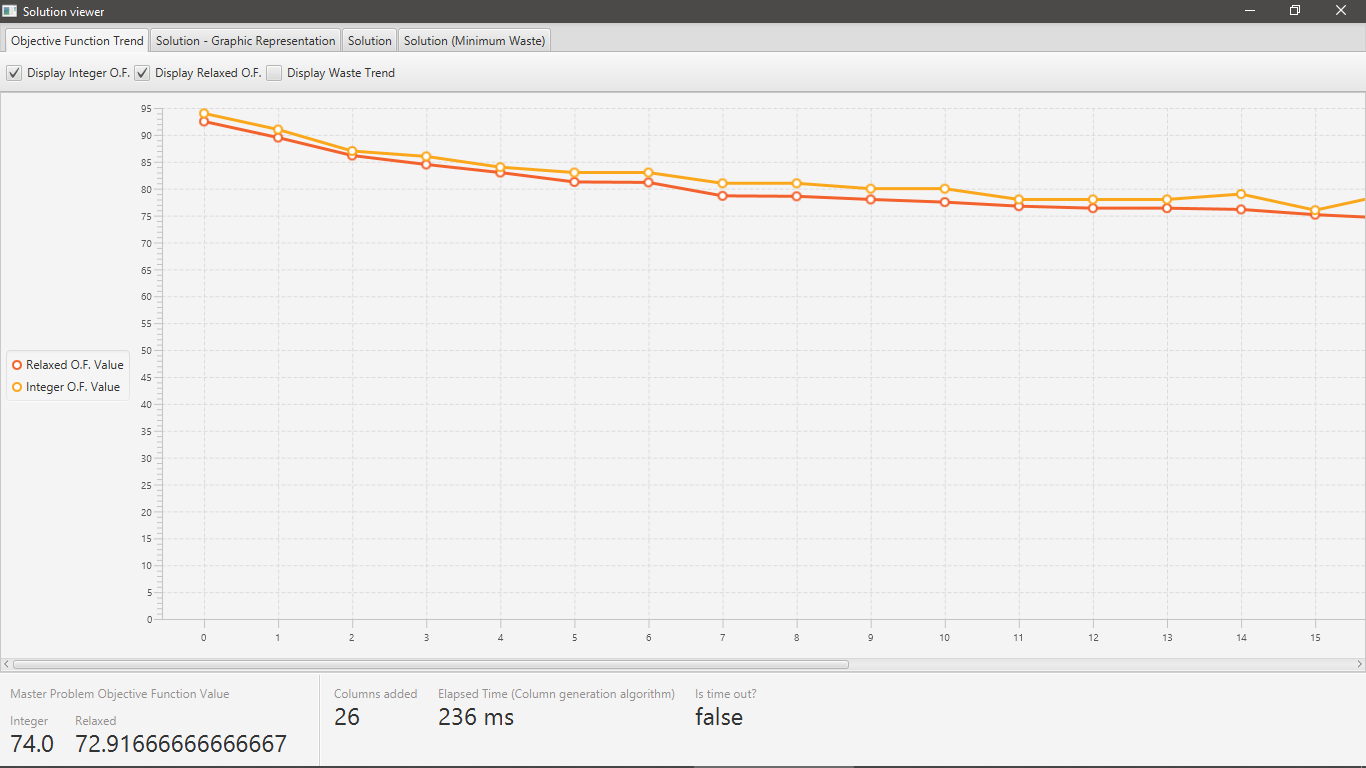
\includegraphics[width=\textwidth]{./images/main.png}
\centering
\caption{Class diagram of our model (main classes and methods only are showed)}

\end{figure}



\begin{figure}[H]
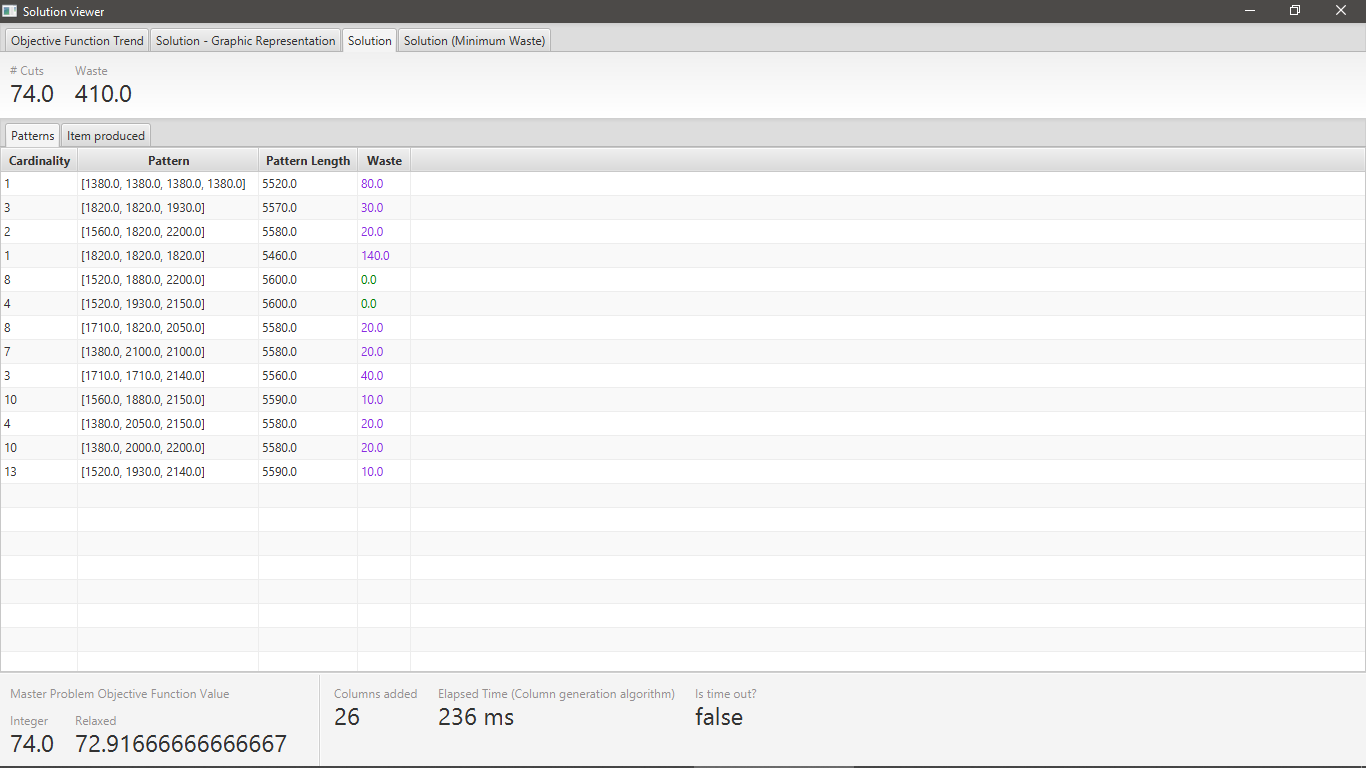
\includegraphics[width=\textwidth]{./images/sol1.png}
\centering
\caption{Class diagram of our model (main classes and methods only are showed)}

\end{figure}


\begin{figure}[H]
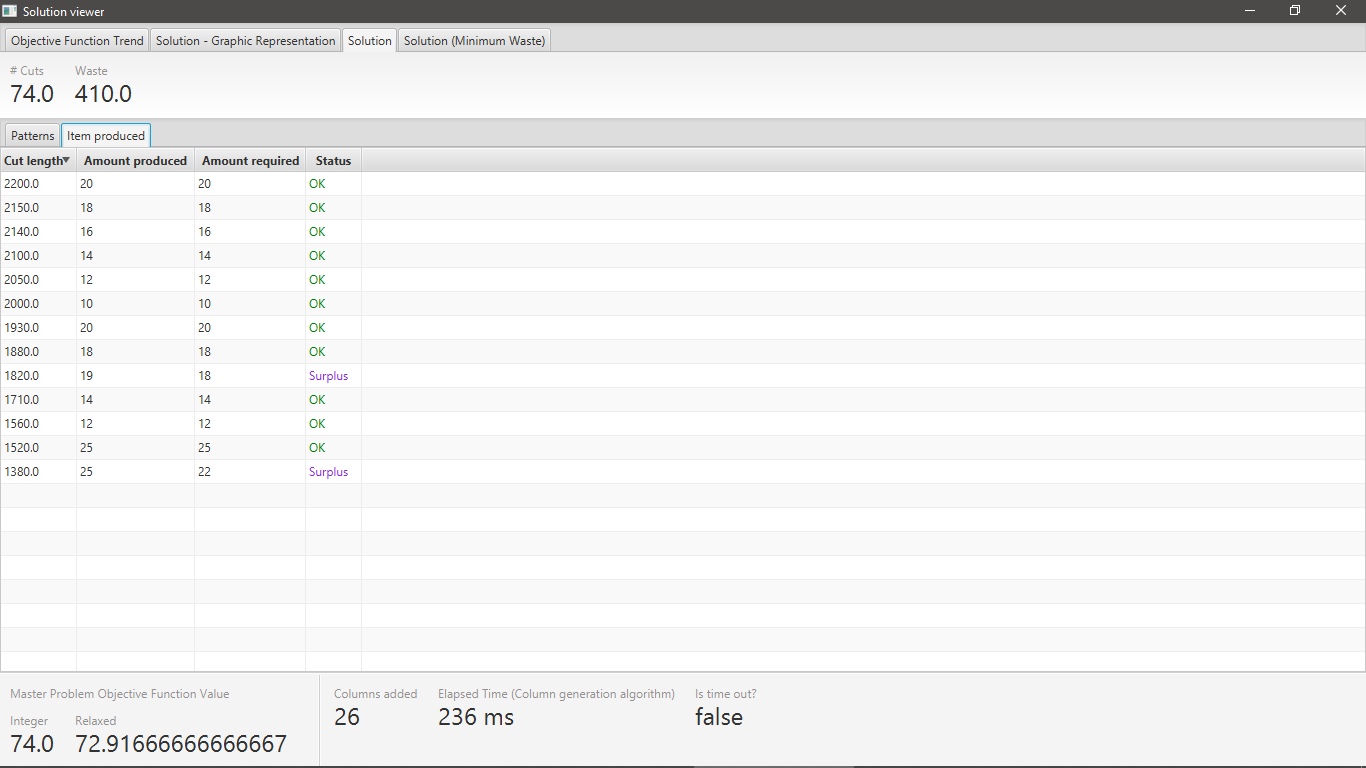
\includegraphics[width=\textwidth]{./images/sol2.png}
\centering
\caption{Class diagram of our model (main classes and methods only are showed)}

\end{figure}

\begin{figure}[H]
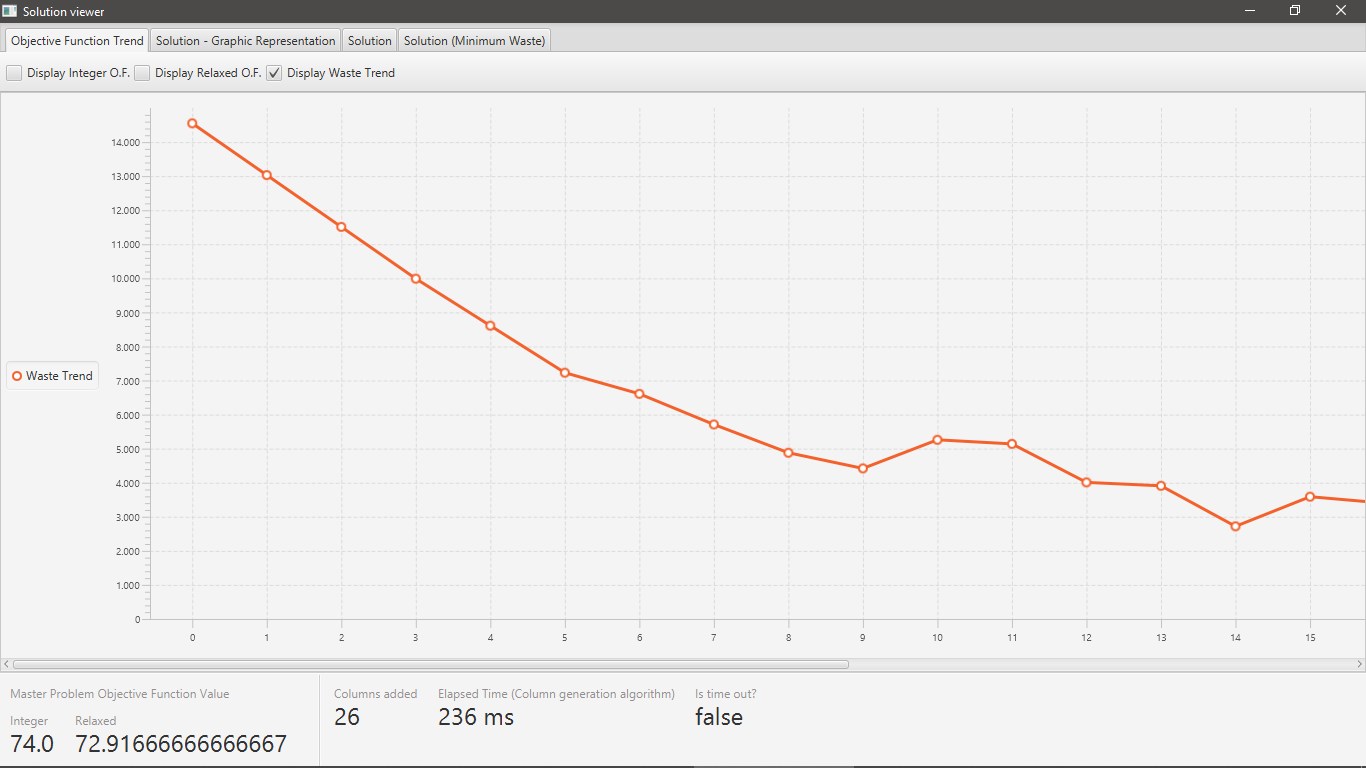
\includegraphics[width=\textwidth]{./images/waste.png}
\centering
\caption{Class diagram of our model (main classes and methods only are showed)}

\end{figure}

\begin{figure}[H]
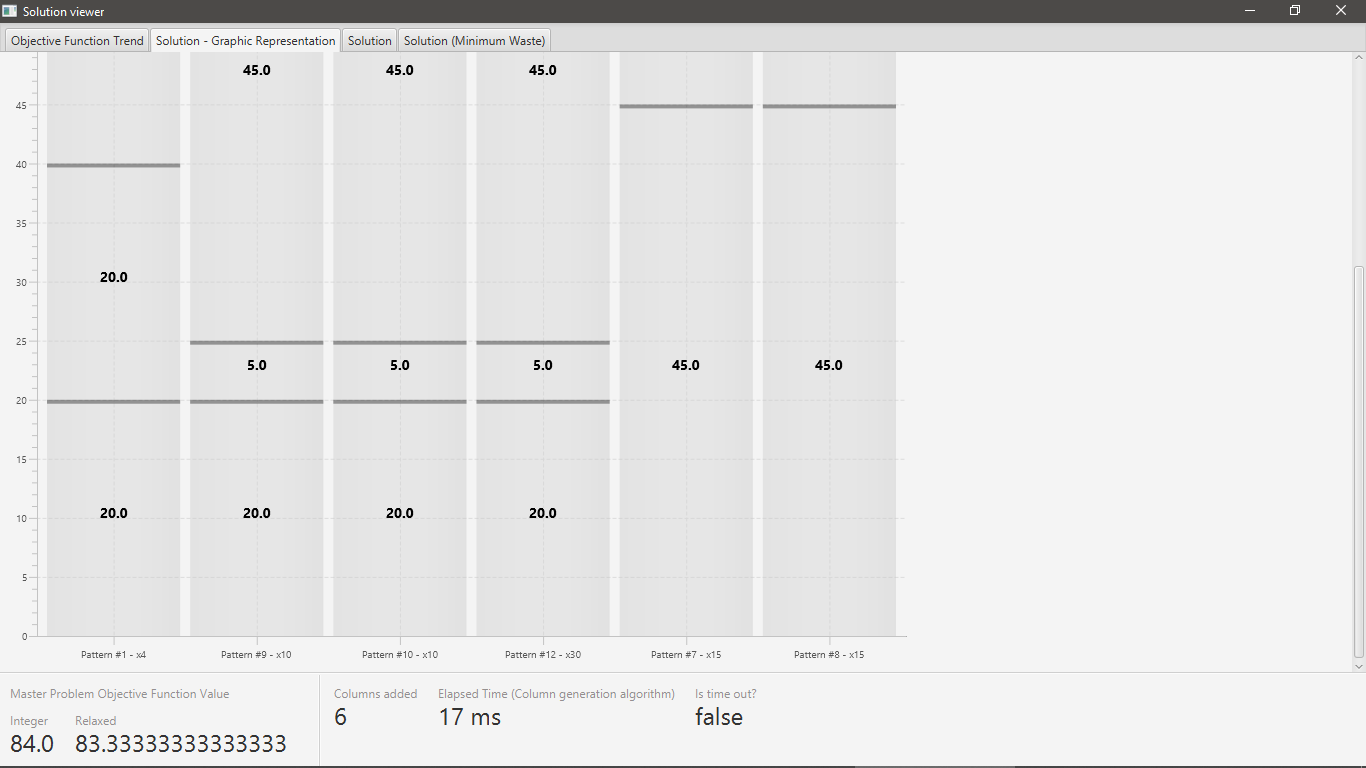
\includegraphics[width=\textwidth]{./images/solgraphic.png}
\centering
\caption{Class diagram of our model (main classes and methods only are showed)}

\end{figure}




\end{document}